\chapter{Meilenstein I}
\label{cha:ms1}

Für den ersten Meilenstein soll ein Programm entwickelt werden, welches auf den Status eines Fotowiderstandes (engl. Light Dependent Resistor, kurz LDR) reagiert. Beim Abdunkeln des LDR wird die LED eingeschaltet, während sie beim Aufhellen deaktiviert wird. Bei der Umsetzung dieser Funktionalität sind die speziellen Charakteristiken der (im vorherigen Kapitel vorgestellten) elektrischen Bauteile zu beachten und in die Planung miteinzubeziehen. Im Folgenden werden die dazu benötigten Vorbetrachtungen in Arbeitsschritten zusammengefasst. 


\section{LED}

Im ersten Schritt soll eine LED per GPIO des Raspberry Pi angesteuert werden. Wie in Kapitel \ref{cha:components} beschrieben, sollte eine Leuchtdiode in Reihe mit einem Vorwiderstand betrieben werden um die Spannung über diese zu begrenzen. 


Die GPIO's des Raspberry Pi stellen 3,3V bei 16mA zur Verfügung. Die Spezifikation der verwendeten LED kann aus der Kennlinie im jeweiligen Datenblatt bestimmt werden. In Bild \ref{img:led_spez} ist der Arbeitspunkt im Strom/Spannungsdiagramm einer grünen LED eingetragen. Man kann erkennen, dass die Durchflussspannung bei gegebenen $16mA$ Strom ca. $2,2V$ beträgt. Bild \ref{img:led_rv} zeigt die zu berechnende Schaltung bei gegebener Spannung $U_0 = 3,3V$ und Strom $I = 16mA$, der gesuchte Vorwiderstand $R_V$ berechnet sich aus dem ohmschen Gesetzt \ref{equ:uri}. \\
\\
Der Gesamtwiderstand einer Reihenschaltung ist die Summe der Einzelwiderstände wie in Gleichung \ref{equ:rgesamt}, genauso ergibt sich die Gesamtspannung aus der Summe der Spannungen über die einzelnen Bauelemente. In diesem Fall gilt: $3,3V = U_{LED} + U_{R_V}$. Aus der Kennlinie der Diode wurde $U_{LED} = 2,2V$ abgelesen. Umstellen des ohmschen Gesetzes ergibt Gleichung \ref{equ:rv} zur Berechnung des Vorwiderstandes. Diese Werte ergeben einen  Vorwiderstand von $68,75 \Omega$. Da i.d.R. nicht so spezifisch hergestellt werden, wird der nächstgrößere Widertstand mit $100 \Omega$ verwendet. Mit Hilfe der pi4j-Bibliothek wird ein Pin für die Ansteuerung der LED konfiguriert wie in Codebeispiel \ref{code:ledcontrol} gezeigt.

\begin{equation}
U = R * I
\label{equ:uri}
\end{equation}

\begin{equation}
R_{Gesamt} = \sum_i^n R_i
\label{equ:rgesamt}
\end{equation}

\begin{figure}
	\centering
	\subfigure[Arbeitspunkt in Kennlinie für grüne LED]{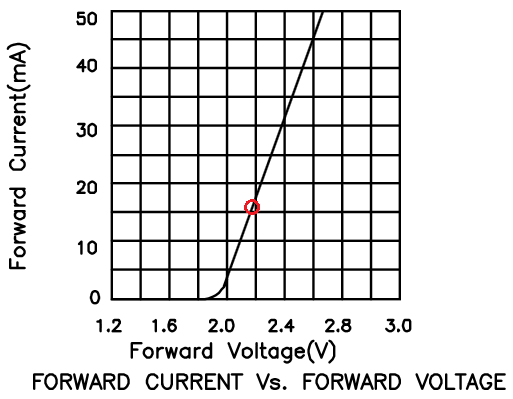
\includegraphics[width=0.45\textwidth]{figures/Schaltplaene/led_spez_ap.png}
	\label{img:led_spez}}
	\subfigure[Reihenschaltung LED und Vorwiderstand $R_V$]{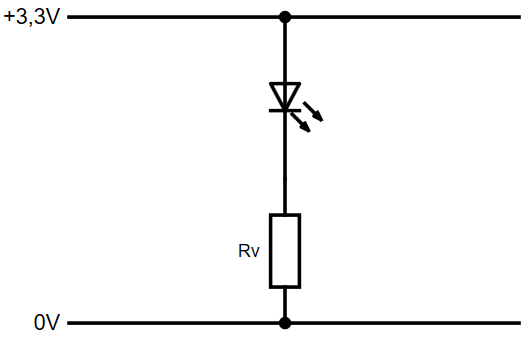
\includegraphics[width=0.45\textwidth]{figures/Schaltplaene/led.png}
	\label{img:led_rv}}
	\caption{Arbeitspunkt und Reihenschaltung einer Leuchtdiode}
	\addloflink{https://kingbright-europe.de/}
\end{figure}


%\begin{figure}
%	\centering
%	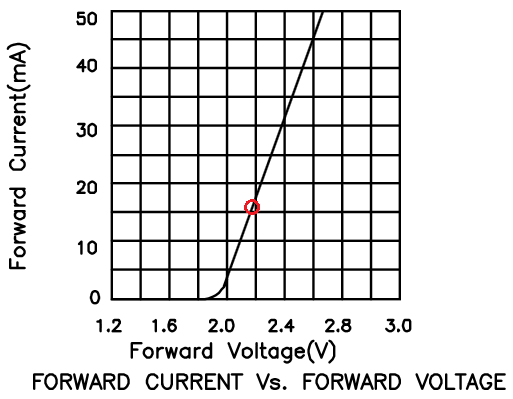
\includegraphics[width=0.5\textwidth]{figures/Schaltplaene/led_spez_ap.png}
%	\caption{Arbeitspunkt in Kennlinie für grüne LED}
%	\label{img:led_spez}
%\end{figure}
%
%\begin{figure}
%	\centering
%	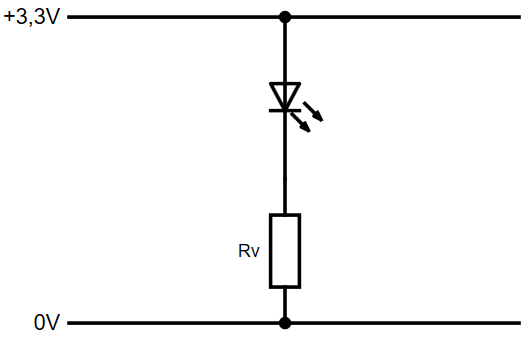
\includegraphics[width=0.45\textwidth]{figures/Schaltplaene/led.png}
%	\caption{Reihenschaltung LED und Vorwiderstand $R_V$}
%	\label{img:led_rv}
%\end{figure}

\begin{equation}
R_V = \frac{U_{R_V}}{I}
\label{equ:rv}
\end{equation}

\begin{lstlisting}[float=htb,caption={Ansteuerung einer LED mittels GPIO},label=code:ledcontrol]
public class LedControl {
  public static void main(String[] args) throws InterruptedException {

    // get a handle to the GPIO controller
	final GpioController gpio = GpioFactory.getInstance();

    // creating the pin with parameter PinState.HIGH
	// will instantly power up the pin
	final GpioPinDigitalOutput pin = gpio.provisionDigitalOutputPin(RaspiPin.GPIO_25, "PinLED", PinState.HIGH);
	System.out.println("light is: ON");

	// wait 2 seconds
	Thread.sleep(2000);

	// turn off GPIO 1
	pin.low();
	System.out.println("light is: OFF");
	// wait 1 second
	Thread.sleep(1000);
	// turn on GPIO 1 for 1 second and then off
	System.out.println("light is: ON for 1 second");
	pin.pulse(1000, true);

	// turn on GPIO 1
	pin.high();
	System.out.println("light is: ON");
		
	// release the GPIO controller resources
	gpio.shutdown();
	}
}
\end{lstlisting}


\section{LDR Digital}

Im zweiten Schritt soll der digitale Wert des LDRs mit dem Raspberry Pi ausgelesen werden. Damit kann erkannt werden, ob es gerade hell oder dunkel ist. Bei einer dunklen Umgebung weist der LDR einen Widerstand von  $10 k \Omega$ und in einer hellen Umgebung einen Widerstand von  $1 k \Omega$ auf. Da der Raspberry Pi für Spannungen $<0,8V$ eine logische 0 und für Spannungen $> 2,0V$ eine logische 1 erkennt, nehmen wir einen Spannungsteiler zur Hilfe. Der korrekte Widerstand lässt sich mit Hilfe der Formel \ref{equ:Spannungsteiler} berechnen:

\begin{equation}
\frac{U_{Ges}}{R_{Ges}} = \frac{U_1 + U_2}{R_1 + R_2} = \frac{U_1}{R_1} = \frac{U_2}{R_2}
\label{equ:Spannungsteiler}
\end{equation}

So lässt sich nun einmal der benötigte Widerstand berechnen, für den Fall, dass der Raspberry Pi eine logische 0 erhalten soll und der LDR eine dunkle Umgebung erkennt:
\begin{equation}
 \frac{U_1}{R_1} = \frac{U_2}{R_2}
\label{equ:vereinfacht}
\end{equation}

Mit den Werten eingesetzt ergibt sich somit die Formel aus \ref{equ:LDR_dunkel}.

\begin{equation}
 \frac{1,3V}{R_1} = \frac{2,0V}{10k \Omega}
\label{equ:LDR_dunkel}
\end{equation}

Analog können wir den benötigten Widerstand für die Helligkeit berechnen, so dass die Spannung im Bereich von $> 2,0V$ liegt und der Raspberry Pi eine logische 1 erkennt (\ref{equ:LDR_hell}).
\begin{equation}
 \frac{2,5V}{R_1} = \frac{0,8V}{1k \Omega}
\label{equ:LDR_hell}
\end{equation}

Löst man die beiden Gleichungen auf, so erhält man das Ergebnis, dass unser Widerstand zwischen $6,5 k \Omega$ und $3,125 k \Omega$ liegen muss. Wir haben daher einen Widerstand von $4.7 k \Omega$ gewählt. Die Schaltung ist in Abbildung \ref{img:plan_1_4_3}  veranschaulicht.

\begin{figure}
	\centering
	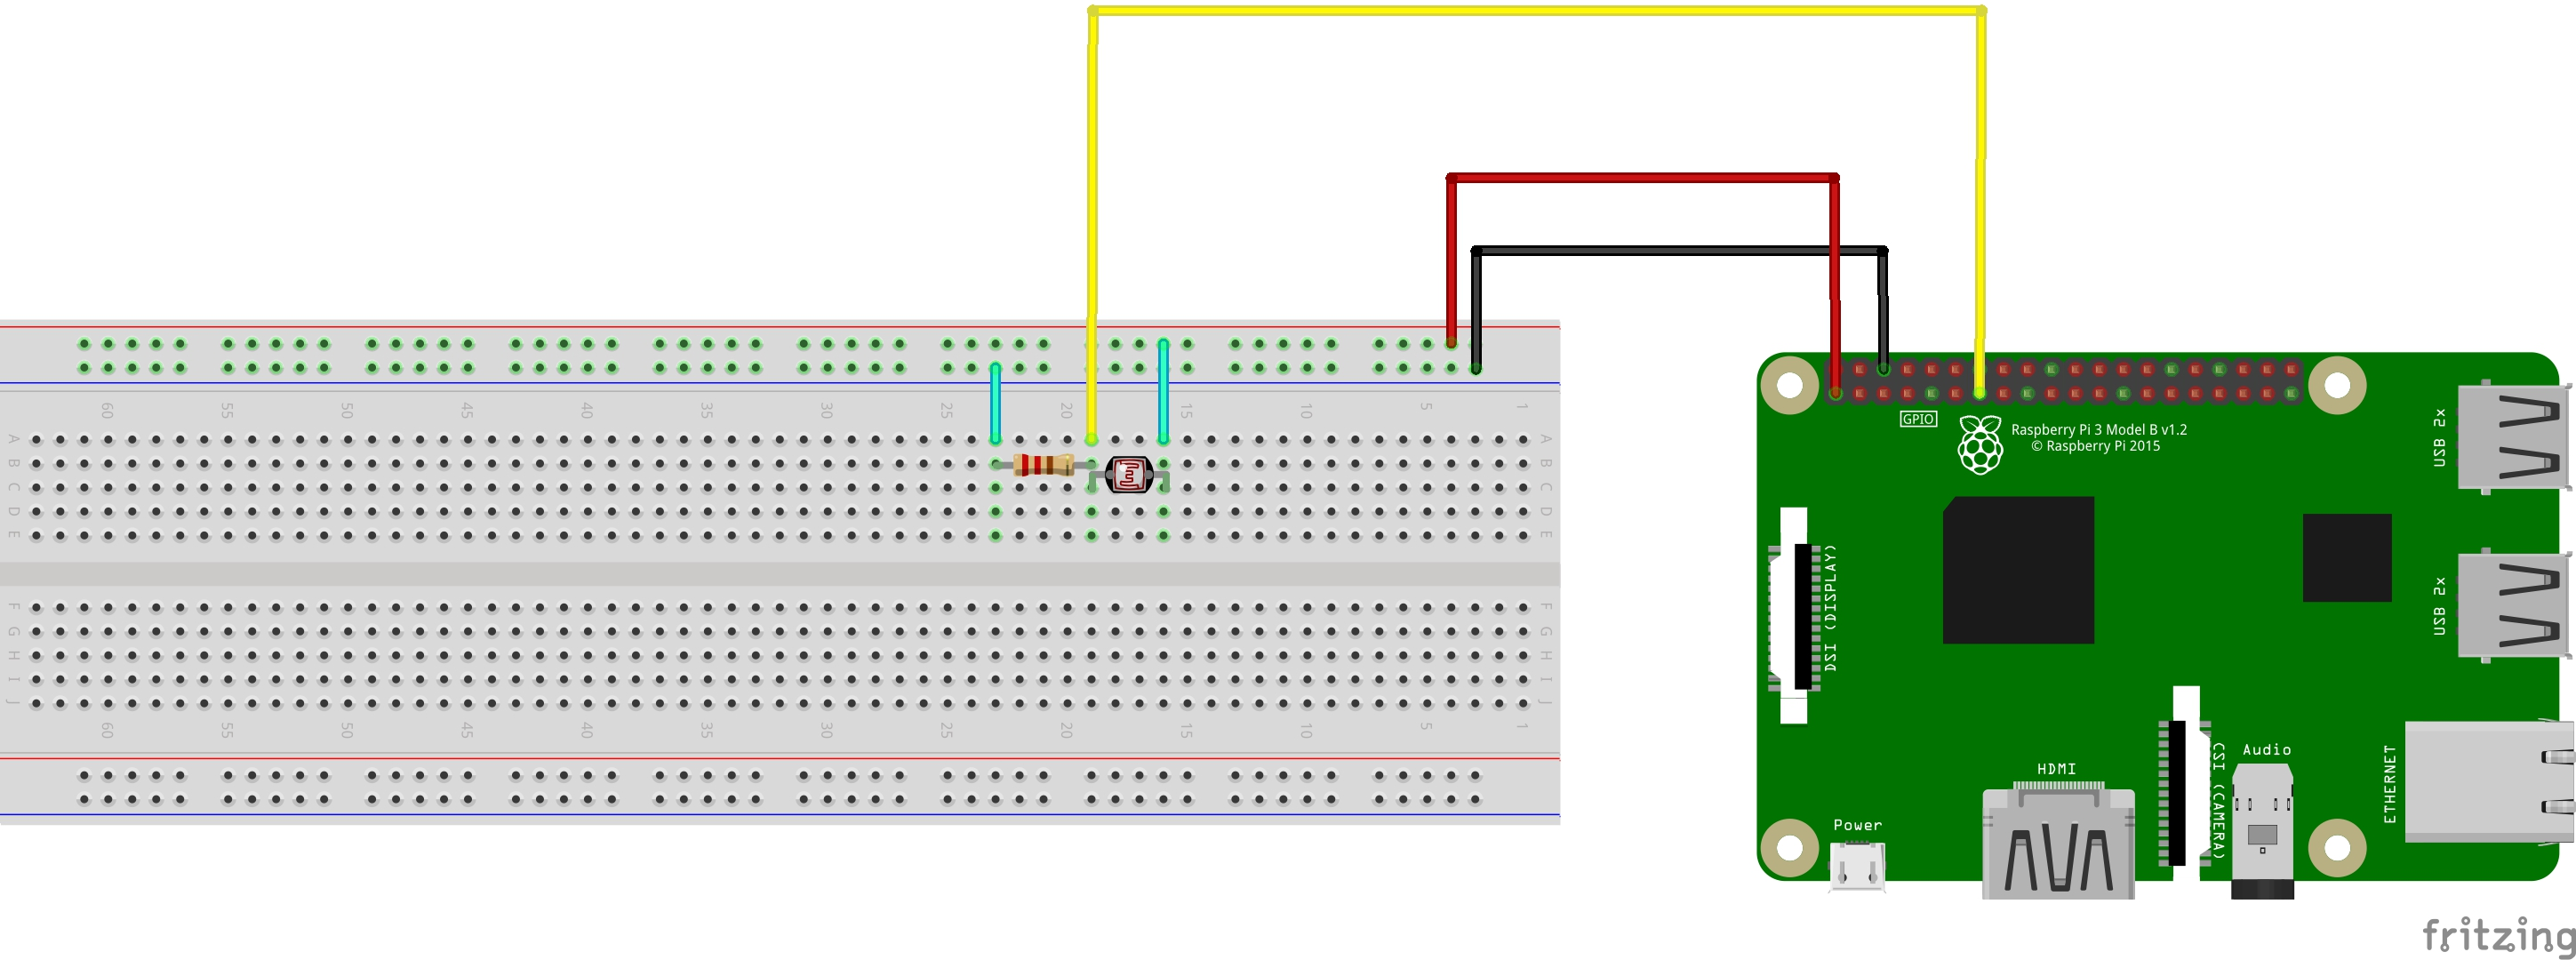
\includegraphics[width=0.5\textwidth]{figures/Schaltplaene/Milestone1_4_3_Steckplatine.jpg}
	\caption{Realisierung der Verbindung des LDR mit dem Raspberry Pi}
	\label{img:plan_1_4_3}
\end{figure}

Den Wert des GPIOs mittels WiringPi lässt sich nun durch den Befehl \ref{code:LDR_digital} auslesen, wobei der GIOP 2 verwendet wurde.

\begin{lstlisting}[caption={Auslesen des GPIOs mittels WiringPi},label=code:LDR_digital]
gpio read 2
\end{lstlisting}

Je nach Beleuchtung wird nun eine 0 für dunkel und eine 1 für hell zurückgeliefert.



\section{LDR Analog}

In diesem Abschnitt des Meilensteins wird der Widerstandswert des Fotowiderstands mit dem im Arduino verbauten A/D-Wandler ausgelesen und in den korrespondierenden Lux-Wert umgerechnet. Wie in Bild \ref{img:adwandler} gezeigt wird ein Spannungsteiler mit Abgriff über den Fotowiderstand konstruiert. Der analoge Eingang am Arduino ist damit in der Lage die über den LDR abfallende Spannung zu bestimmen. Der 10-Bit A/D-Wandler des Arduino gibt Werte zwischen $0-1023$ aus, daher berechnet sich die über den LDR abfallende Spannung wie in Gleichung \ref{equ:adwandler} beschrieben. Der entsprechende Widerstand ergibt sich durch Umstellen der Spannungsteilerformel zu Gleichung \ref{equ:spannungsteiler}. In Codebeispiel \ref{code:analogread} wird gezeigt wie der Wert des Fotowiderstandes mittels analogem Pin am Arduino ausgelesen wird. Schließlich soll Wert des Fotowiderstandes noch in den entsprechenden Lux-Wert umgerechnet werden. Zu diesem Zweck wird das nichtlineare Kennlinienverhalten des Fotowiderstandes linearisiert, wie in Bild \ref{img:ldr_kennlinie} dargestellt ist. Hier werden die zwei Punkte $P1: 6k\Omega, 50Lux$ und $P2: 50k\Omega, 2Lux$ gewählt und damit eine Geradengleichung \ref{equ:geradengleichung} zur Approximation des Lux-Wertes konstruiert. Die logarithmische Darstellung des Widerstandsverhaltens erfordert eine Anpassung in der Geradengleichung die in Gleichung \ref{equ:loggerade} beschrieben ist. Durch Einsetzen der gewählten Punkte lassen sich Steigung und Offset der Gerade zu \ref{equ:line_m} und \ref{equ:line_n} berechnen und die Gleichung zur Umrechnung in Lux-Wert aufstellen \ref{equ:luxgleichung}. 

\begin{equation}
U_{LDR} = \frac{analogValue * U_{IN}}{1023}
\label{equ:adwandler}
\end{equation}

\begin{equation}
R_{LDR}=\frac{R_V * U_{LDR}}{U_{IN} - U_{LDR}}
\label{equ:spannungsteiler}
\end{equation}

\begin{equation}
f(x)=m*x+n
\label{equ:geradengleichung}
\end{equation}

\begin{equation}
ln(E_{Lux})=m*ln(R_{LDR})+n
\label{equ:loggerade}
\end{equation}

\begin{equation}
\begin{split}
m = \frac{ln(50)-ln(2)}{ln(6)-ln(50)} = -1.5181489
\end{split}
\label{equ:line_m}
\end{equation}

\begin{equation}
n = ln(50) - m*ln(6) = 6.6321807
\label{equ:line_n}
\end{equation}

\begin{equation}
E_{Lux} = R_{LDR}^{-1.5181489}*759.1358
\label{equ:luxgleichung}
\end{equation}

\begin{figure}
	\centering
	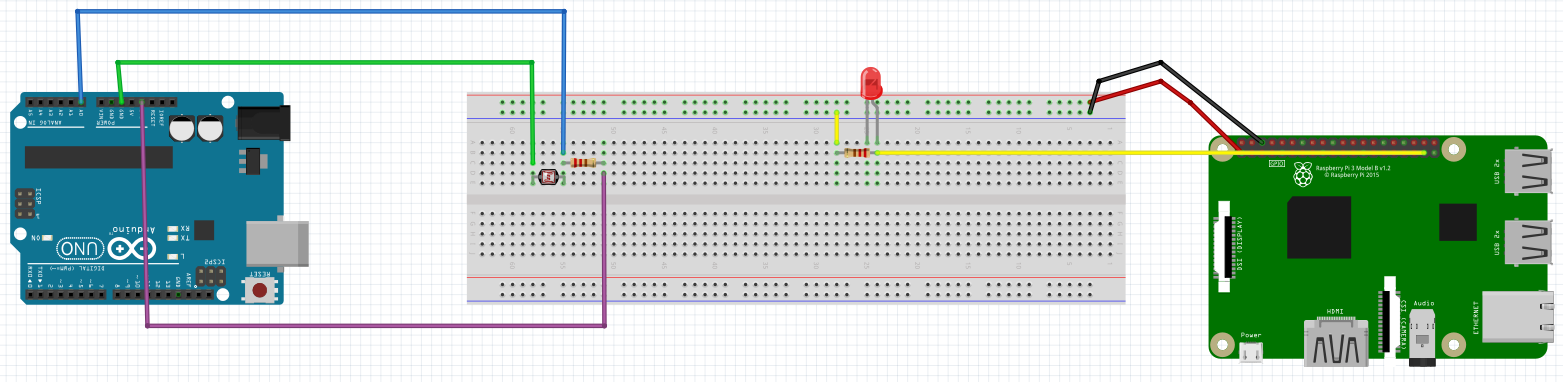
\includegraphics[width=0.85\textwidth]{figures/Schaltplaene/adwandler.png}
	\caption{Spannungsteiler mit Abgriff am Fotowiderstand}
	\label{img:adwandler}
\end{figure}

\begin{figure}
	\centering
	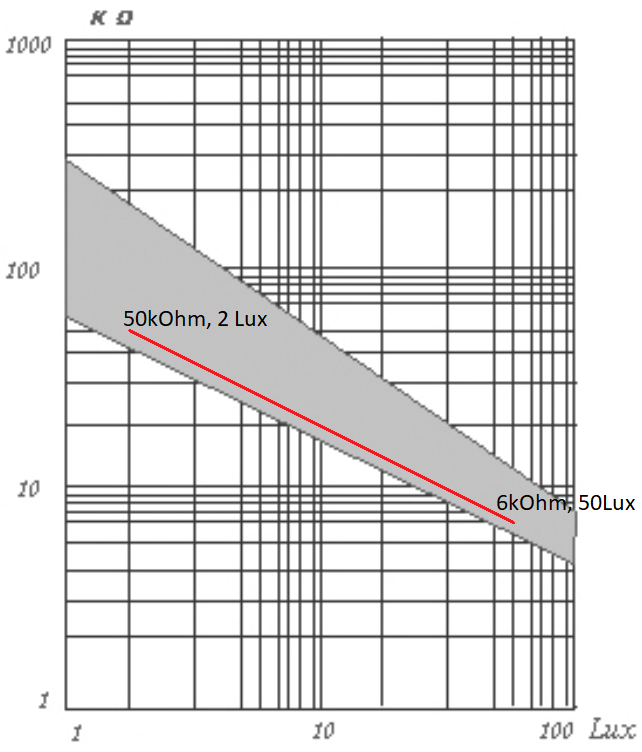
\includegraphics[width=0.85\textwidth]{figures/ldr_kennlinie.png}
	\caption{Widerstandscharakteristik LDR mit Liniearisierungsgeraden}
	\addloflink{https://kingbright-europe.de/}
	\label{img:ldr_kennlinie}
\end{figure}


\begin{lstlisting}[float=htb,caption={Auslesen des analogen LDR Widerstandswertes und Umrechnung in Lux},label=code:analogread]
#include <Wire.h>
#include <math.h>

int sensorPin = 0;
int ledPin = 13;
int sensorValue = 0;

const float u_in = 5.0; // input voltage in volt
const float r_v = 4.7; // reference resistor in ohm
const float pow_factor = -1.31022; // calculated value for lux estimation
const float l_factor = 210.9143;

float u_ldr = 0.0;  // voltage over light sensor
float r_ldr = 0.0;  // resistance of light sensor
float e_v = 0.0;    // Lux value measured

void setup() {
  // start serial communication
  Serial.begin(9600);
}

// main function repeated in a loop
void loop() {
  // readout sensor Pin
  sensorValue = analogRead(sensorPin);

  u_ldr = ((sensorValue * u_in) / 1023);
  r_ldr = ((r_v * u_ldr) / (u_in - u_ldr));
  e_v = (pow(r_ldr, pow_factor)) * l_factor;
  
  // send calulated lux-value
  Serial.println(e_v);
  delay(2000);
}
\end{lstlisting}

\begin{lstlisting}[float=htb,caption={Initialisierung der seriellen Schnittstelle im Raspberry Pi, \quelle\url{http://playground.arduino.cc/Interfacing/Java}},label=code:piserial]
public void initialize() {
  System.setProperty("gnu.io.rxtx.SerialPorts", "/dev/ttyACM0");
  CommPortIdentifier portId = null;
  Enumeration portEnum = CommPortIdentifier.getPortIdentifiers();

  //First, Find an instance of serial port as set in PORT_NAMES.
  while (portEnum.hasMoreElements()) {
	CommPortIdentifier currPortId = (CommPortIdentifier) portEnum.nextElement();
	for (String portName : PORT_NAMES) {
	  if (currPortId.getName().equals(portName)) {
		portId = currPortId;
		break;
	  }
	}
  }
  if (portId == null) {
	System.out.println("Could not find COM port.");
	return;
  }
  try {
	// open serial port, and use class name for the appName.
	serialPort = (SerialPort) portId.open(this.getClass().getName(),
		TIME_OUT);
	// set port parameters
	serialPort.setSerialPortParams(DATA_RATE,
	SerialPort.DATABITS_8,
	SerialPort.STOPBITS_1,
	SerialPort.PARITY_NONE);
	// open the streams
	input = new BufferedReader(new InputStreamReader(serialPort.getInputStream()));
	output = serialPort.getOutputStream();
	// add event listeners
	serialPort.addEventListener(this);
	serialPort.notifyOnDataAvailable(true);
  } catch (Exception e) {
    System.err.println(e.toString());
  }
}
\end{lstlisting}

Die Kommunikation zwischen Raspberry Pi und Arduino erfolgt über die serielle Schnittstelle. Dazu wird der Arduino mittel USB Kabel an den Raspberry Pi angeschlossen. Im Codebeispiel \ref{code:analogread} ist zu erkennen, dass der Ardunio die serielle Kommunikation mit 9600 Baud startet und den Wert des LDR alle 2 Sekunden ausliest und auf den Kanal legt. Auf Seiten des Raspberry Pi wird die serielle Schnittstelle mit Hilfe der RXTX-Bibliothek angesprochen. Die Initialisierung der seriellen Schnittstelle ist in Codebeispiel \ref{code:piserial} beschrieben. Das Senden eines Wertes erzeugt im Raspberry Pi ein Event auf dem seriellen Port, in Codebeispiel \ref{code:piserialread} ist dargestellt wie der Pi auf solch ein Event reagiert. In diesem Fall wird die LED aktiviert wenn der empfangene Wert größer als ein definierter Grenzwert ist und sonst deaktivert.

\begin{lstlisting}[float=htb,caption={Auslesen der seriellen Schnittstelle im Raspberry Pi, \quelle\url{http://playground.arduino.cc/Interfacing/Java}},label=code:piserialread]
public synchronized void serialEvent(SerialPortEvent oEvent) {
  if (oEvent.getEventType() == SerialPortEvent.DATA_AVAILABLE) {
    try {
      double inputLine=Double.parseDouble(input.readLine());
	  if (inputLine > Threshold) pin.high;
	  else pin.low;
	  
	} catch (Exception e) {
	  System.err.println(e.toString());
	}
  }
}
\end{lstlisting}


%The following is just a further quick link list compiled to help in creating good scientific presentations.
%\begin{itemize}
%\item \url{http://www.the-scientist.com/?articles.view/articleNo/28818/title/Pimp-your-PowerPoint/}
%\item \url{http://www.northwestern.edu/climb/resources/oral-communication-skills/creating-a-presentation.html}
%\item \url{http://www.nextscientist.com/improve-presentation-skills-of-phd-students/}
%\end{itemize}


%%%%% Emacs-related stuff
%%% Local Variables: 
%%% mode: latex
%%% TeX-master: "../../main"
%%% End: 
